\documentclass[10pt]{article}
\usepackage[spanish]{babel}
\usepackage[a4paper, tmargin=0.75in, lmargin=0.80in, rmargin=0.80in, bmargin=1in]{geometry}
\usepackage{hyperref}
\usepackage{float}
%\usepackage{multicol}
\hypersetup{
    colorlinks=true,
    linkcolor=black,
    filecolor=magenta,      
    urlcolor=blue,
    citecolor=black,
}
\usepackage{graphicx}
\usepackage{amsfonts}
\usepackage{amsthm}
\usepackage{amssymb}
\usepackage{lipsum}
\usepackage{amsmath}
\usepackage{tabularx}
\usepackage{pdflscape}
\usepackage{booktabs}
\usepackage{bbm}
\usepackage{listings}
\usepackage{xcolor}

\usepackage[
  backend=biber,
  style=alphabetic,
  citestyle=alphabetic,
  doi=true,
  url=true,
  isbn=false,
  eprint=false,
  maxbibnames=99
]{biblatex}

\addbibresource{referencias.bib}

% Definimos colores estilo "terminal con fondo negro"
\definecolor{backcolour}{rgb}{0.1,0.1,0.1}
\definecolor{codegreen}{rgb}{0,0.8,0}
\definecolor{codegray}{rgb}{0.7,0.7,0.7}
\definecolor{codepurple}{rgb}{0.8,0.6,1}
\definecolor{codewhite}{rgb}{1,1,1}


\lstdefinestyle{mypython}{
    backgroundcolor=\color{backcolour},
    basicstyle=\ttfamily\scriptsize\color{codewhite},
    commentstyle=\color{codegreen},
    keywordstyle=\color{codepurple},
    stringstyle=\color{codegreen},
    numbers=left,
    numberstyle=\tiny\color{codegray},
    breaklines=true,
    breakatwhitespace=false,
    showstringspaces=false,
    tabsize=4
}

\lstset{style=mypython}







\pagestyle{empty}


%%%%%%%%%%%%%%%%%%%%%%%%%%%%%%%%%%%%%%%%%%%%%%%%%%
%%%%%%%%%%%%%%%%%%%%%%%%%%%%%%%%%%%%%%%%%%%%%%%%%%
%%%%%%%%%%%%%%%%%%%%%%%%%%%%%%%%%%%%%%%%%%%%%%%%%%
%%%%%%%%%%%%%%%%%%%%%%%%%%%%%%%%%%%%%%%%%%%%%%%%%%
% ENTER SOME IMPORTANT INFORMATION
%%%%%%%%%%%%%%%%%%%%%%%%%%%%%%%%%%%%%%%%%%%%%%%%%%
%%%%%%%%%%%%%%%%%%%%%%%%%%%%%%%%%%%%%%%%%%%%%%%%%%
%%%%%%%%%%%%%%%%%%%%%%%%%%%%%%%%%%%%%%%%%%%%%%%%%%
%%%%%%%%%%%%%%%%%%%%%%%%%%%%%%%%%%%%%%%%%%%%%%%%%%
\newcommand{\studentname}{Sánchez, Hazel; Hernández, Debany ; Canché, Elías}
\newcommand{\researchcentre}{Maestría en Probabilidad y Estadística}
\newcommand{\institution}{Centro de Investigación en Matemáticas (CIMAT)}
\newcommand{\projecttitle}{Tarea 2}
\newcommand{\supervisor}{Dr. Marco Antonio Aquino López}
%%%%%%%%%%%%%%%%%%%%%%%%%%%%%%%%%%%%%%%%%%%%%%%%%%
%%%%%%%%%%%%%%%%%%%%%%%%%%%%%%%%%%%%%%%%%%%%%%%%%%
%%%%%%%%%%%%%%%%%%%%%%%%%%%%%%%%%%%%%%%%%%%%%%%%%%
%%%%%%%%%%%%%%%%%%%%%%%%%%%%%%%%%%%%%%%%%%%%%%%%%%
%%%%%%%%%%%%%%%%%%%%%%%%%%%%%%%%%%%%%%%%%%%%%%%%%%
%%%%%%%%%%%%%%%%%%%%%%%%%%%%%%%%%%%%%%%%%%%%%%%%%%

\begin{document}

\begin{center}
{\Large{Proyecto 2: Clasificación Supervisada}} \\
\vspace{2mm}
{\Large{Introducción a la Ciencia de Datos}} \\
\end{center}

\vspace{5mm}
\hrule
\vspace{1mm}
\hrule

\vspace{3mm}
\begin{tabular}{ll} 
Integrantes:           	        & {\studentname}   \\ 
Programa Educativo: 	        & {\researchcentre}  \\ 
Institución:                 & {\institution}  \\
Profesor: 	                 & {\supervisor}  \\ 
\end{tabular}

\vspace{3mm}
\hrule
\vspace{1mm}
\hrule

\begin{abstract}

\end{abstract}
\section{Análisis computacional mediante simulaciones (Segunda Parte de la Tarea)}

\subsection*{Introducción}


En esta segunda parte se busca analizar, en un entorno controlado, el desempeño de distintos clasificadores supervisados frente al clasificador óptimo de Bayes. A diferencia de la primera parte, donde el análisis se realizó sobre datos reales del \textit{Bank Marketing Dataset}, aquí se emplean datos sintéticos generados a partir de distribuciones normales multivariadas con parámetros conocidos, lo que permite calcular de manera exacta el riesgo de Bayes y utilizarlo como referencia teórica.

El marco de simulación implementado permite estudiar diversos escenarios que reflejan condiciones típicas en problemas de clasificación. En particular, se consideraron: 
\begin{itemize}
\item[i)] clases con covarianzas iguales, donde el clasificador lineal discriminante (LDA) coincide con el óptimo de Bayes, 

\item[ii)] clases con covarianzas distintas, donde el clasificador cuadrático discriminante (QDA) coincide con Bayes, y 

\item[iii)] situaciones de balance y desbalance en las probabilidades a priori de las clases. 
\end{itemize}
Además, se evaluaron diferentes grados de solapamiento entre distribuciones mediante la elección de medias y covarianzas, con el fin de analizar casos fáciles, intermedios y difíciles de clasificar.

Los métodos comparados incluyen: el clasificador de Bayes (óptimo), Naive Bayes gaussiano, LDA, QDA, el criterio de Fisher (proyección en una dimensión con umbral) y el algoritmo de k-vecinos más cercanos (k-NN) con distintos valores de $k$. La comparación se realizó tanto en términos de riesgo verdadero, calculado directamente a partir de las distribuciones, como en términos de riesgo estimado mediante validación cruzada estratificada sobre los datos simulados. Esta doble perspectiva permite contrastar el comportamiento teórico con el desempeño observado bajo técnicas prácticas de validación.

El diseño experimental incluyó variaciones en el tamaño muestral ($n \in \{50, 100, 200, 500\}$ por clase) y en el hiperparámetro de k-NN ($k \in \{1, 3, 5, 11, 21\}$), así como réplicas Monte Carlo para promediar resultados y obtener estimadores estables de riesgo. Se generaron tablas y gráficas que muestran la evolución de los riesgos, las brechas respecto a Bayes y la comparación entre validación y riesgo verdadero. 

En suma, esta sección tiene como finalidad no solo cuantificar las diferencias de desempeño entre los clasificadores, sino también reflexionar sobre las condiciones que favorecen o limitan su eficacia, conectando la teoría estadística de clasificación con la evidencia empírica obtenida mediante simulación computacional.

\subsection*{Metodología}
\paragraph{Modelo de generación de datos.}
Se consideraron dos clases $Y \in \{0,1\}$, con probabilidades a priori $\pi_0$ y $\pi_1$ (por defecto $\pi_0=\pi_1=0.5$, aunque también se analizaron escenarios desbalanceados como $\pi_0=0.8$, $\pi_1=0.2$).  
Dado $Y=k$, los predictores $X \in \mathbb{R}^p$ siguen una distribución normal multivariada:
\[
X \mid Y=k \sim \mathcal{N}_p(\mu_k, \Sigma_k).
\]

Los parámetros $(\mu_k, \Sigma_k)$ se fijaron de manera que permitieran reproducir condiciones de clasificación:
\begin{itemize}
    \item \textbf{Clases bien separadas}: medias distantes y covarianzas con baja correlación.
    \item \textbf{Clases intermedias}: medias cercanas con solapamiento moderado.
    \item \textbf{Clases difíciles}: medias muy próximas y covarianzas grandes o altamente correlacionadas.
\end{itemize}

Se trabajó principalmente con $p=2$ (dos dimensiones) para facilitar la visualización de las fronteras de decisión y la interpretación geométrica. Este diseño permite verificar gráficamente cómo cambian las regiones de clasificación bajo cada método.

\paragraph{Escenarios analizados.}
Se plantearon cuatro configuraciones experimentales principales:
\begin{enumerate}
    \item \textbf{Covarianzas iguales y datos balanceados}. Aquí $\Sigma_0 = \Sigma_1$, y por teoría estadística el clasificador de Bayes coincide con LDA. Es el escenario más “favorable” para LDA.
    \item \textbf{Covarianzas distintas y datos balanceados}. En este caso, $\Sigma_0 \neq \Sigma_1$, por lo que QDA coincide con el clasificador óptimo de Bayes. Se evalúa cómo otros métodos se desvían del óptimo.
    \item \textbf{Covarianzas iguales con clases desbalanceadas}. Con $\pi_0 \neq \pi_1$, se introduce el efecto del desbalance en el error de clasificación. La frontera de Bayes se desplaza según los priors.
    \item \textbf{Covarianzas distintas con clases desbalanceadas}. Combina la dificultad de covarianzas heterogéneas y el desbalance, siendo el escenario más desafiante.
\end{enumerate}

\paragraph{Clasificadores comparados.}
Se implementaron los siguientes métodos, en concordancia con lo visto en clase:
\begin{itemize}
    \item \textbf{Clasificador óptimo de Bayes}: calculado directamente a partir de las densidades gaussianas y priors conocidos.
    \item \textbf{Naive Bayes gaussiano}: asume independencia condicional entre variables y covarianzas diagonales.
    \item \textbf{LDA (Linear Discriminant Analysis)}: utiliza una matriz de covarianza común para ambas clases.
    \item \textbf{QDA (Quadratic Discriminant Analysis)}: permite matrices de covarianza diferentes por clase.
    \item \textbf{Criterio de Fisher}: proyección unidimensional $z=w^\top x$ con $w \propto S_W^{-1}(\mu_1 - \mu_0)$ y clasificación por umbral en el espacio proyectado.
    \item \textbf{k-NN}: clasificación basada en la mayoría entre los $k$ vecinos más cercanos en el espacio euclidiano. Se exploraron valores $k \in \{1, 3, 5, 11, 21\}$.
\end{itemize}

\paragraph{Cálculo del riesgo.}
El desempeño se cuantifica con el riesgo de clasificación:
\[
L(g) = \mathbb{P}(g(X) \neq Y).
\]
Se estimaron dos variantes:
\begin{enumerate}
    \item \textbf{Riesgo verdadero (teórico)}: dado que las distribuciones son conocidas, el error de cada clasificador se estimó con un conjunto de prueba grande ($N \gg 10^4$) generado de la misma distribución. En el caso de Bayes, este valor corresponde al riesgo óptimo.
    \item \textbf{Riesgo estimado por validación}: se utilizó validación cruzada estratificada de 5 pliegues sobre la muestra simulada de entrenamiento, obteniendo un estimador empírico del riesgo. Esto permite comparar la cercanía entre los valores de validación y los riesgos verdaderos.
\end{enumerate}

\paragraph{Diseño experimental.}
El experimento se estructuró de manera que permitiera evaluar de forma justa y sistemática el desempeño de los distintos clasificadores bajo condiciones comparables. Para ello, se plantearon diferentes configuraciones de parámetros y se introdujo un esquema de replicación con el fin de controlar la variabilidad inherente a la simulación Monte Carlo. En detalle, el diseño contempló lo siguiente:

\begin{enumerate}
    \item \textbf{Tamaños muestrales:} se generaron muestras independientes para cada combinación de parámetros $(n,k)$, donde el tamaño muestral por clase se varió en $n \in \{50, 100, 200, 500\}$. Esta elección permite observar la evolución del riesgo conforme aumenta la cantidad de información disponible, capturando desde escenarios con datos escasos hasta contextos más estables.
    
    \item \textbf{Entrenamiento de clasificadores:} en cada réplica simulada se ajustaron todos los métodos (Bayes, Naive Bayes, LDA, QDA, Fisher y k-NN). De esta forma, las comparaciones entre modelos se realizan siempre bajo exactamente las mismas condiciones de datos, garantizando que las diferencias en desempeño provienen del método y no de la muestra.
    
    \item \textbf{Estimación de riesgos:} para cada clasificador se calcularon tanto el riesgo verdadero (a partir de un conjunto de prueba Monte Carlo de gran tamaño) como el riesgo estimado por validación cruzada estratificada. Esta doble evaluación permite contrastar el valor teórico de referencia con el estimador práctico usado en aplicaciones reales, discutiendo posibles sesgos y la variabilidad de cada aproximación.
    
    \item \textbf{Replicación:} el procedimiento anterior se repitió $R=20$ veces por condición experimental. El objetivo es reducir la influencia del azar en cada simulación individual y poder reportar, para cada método, la media y desviación estándar del riesgo. Este enfoque asegura resultados más robustos y facilita la comparación estadística entre modelos.
\end{enumerate}

En conjunto, este diseño experimental equilibra control y variabilidad: por un lado, se fijan parámetros para aislar los factores de interés (n, k, covarianzas, balance de clases) y, por otro, se replican las simulaciones para obtener estimadores estables y confiables del riesgo de clasificación.


\paragraph{Productos obtenidos.}
A partir de la estrategia de simulación descrita, se generaron distintos productos gráficos y numéricos cuyo objetivo es sintetizar el comportamiento de los clasificadores bajo escenarios controlados y facilitar la comparación entre ellos. Cada uno responde a una necesidad particular del análisis:

\begin{itemize}
    \item \textbf{Curvas $L(g)$ vs.\ $n$:} muestran la evolución del riesgo de clasificación conforme aumenta el tamaño de la muestra. Estas gráficas permiten evaluar la rapidez con la que cada método converge hacia su desempeño asintótico y evidencian qué clasificadores requieren más datos para estabilizarse.

    \item \textbf{Curvas $L(\text{k-NN})$ vs.\ $k$:} permiten estudiar la sensibilidad del clasificador k-NN respecto a su hiperparámetro principal. Comparar diferentes valores de $k$ en distintos tamaños muestrales ayuda a identificar el compromiso óptimo entre sesgo y varianza, así como a comprender en qué condiciones k-NN se acerca o se aleja del clasificador de Bayes.

    \item \textbf{Brechas $L(g) - L(\text{Bayes})$:} cuantifican explícitamente la distancia entre cada método y el óptimo teórico. Estas gráficas son particularmente informativas porque muestran no solo el nivel de error absoluto, sino también el “costo” relativo de utilizar un clasificador más simple frente al ideal de Bayes.

    \item \textbf{Comparación validación vs.\ riesgo verdadero:} permite analizar hasta qué punto las estimaciones prácticas obtenidas mediante validación cruzada reflejan el desempeño real esperado bajo las distribuciones conocidas. Esto aporta una reflexión crítica sobre el sesgo y la variabilidad de los métodos de validación más comunes en aplicaciones reales.

    \item \textbf{Tablas de resumen (media $\pm$ desviación estándar):} condensan la información numérica de múltiples réplicas en un formato compacto. Estas tablas facilitan la lectura comparativa entre clasificadores y escenarios, y sirven como apoyo formal para las conclusiones obtenidas a partir de las gráficas.
\end{itemize}

En conjunto, estos productos ofrecen una visión completa del problema: las gráficas capturan las tendencias cualitativas y la dinámica de los clasificadores, mientras que las tablas nos proveen evidencia cuantitativa y precisa. Ambos complementos permiten no solo comparar el desempeño entre métodos, sino también interpretar cómo la naturaleza de los datos y las condiciones experimentales influyen en la calidad de la clasificación.

\paragraph{Reproducibilidad.}
El código se organizó en módulos (\texttt{utils/clasificadores.py}, \texttt{utils/distributions.py}, \texttt{utils/risk\_analysis.py}), centralizando la configuración de parámetros en un archivo \texttt{config.py}. Todas las simulaciones fueron orquestadas desde un \texttt{main.py}, con generación automática de figuras y exportación de resultados. Se fijaron semillas aleatorias para garantizar reproducibilidad y comparabilidad entre réplicas.


\medskip


Con la metodología descrita, se cuenta con un marco experimental completo para evaluar de manera sistemática el desempeño de los clasificadores. El diseño de escenarios, la generación de datos sintéticos y la estrategia de replicación permiten obtener tanto estimaciones teóricas como empíricas del riesgo de clasificación. A continuación, se presentan los resultados obtenidos, organizados por escenario, donde se analizan las diferencias entre los métodos y su distancia respecto al clasificador de Bayes, así como la evolución de su comportamiento bajo cambios en el tamaño muestral, el desbalance y los hiperparámetros.


\subsection*{Comportamiento de clasificadores}

\subsection*{Escenario 1: Clases balanceadas con covarianzas iguales}

En este escenario se fijaron priors balanceados $\pi_0=\pi_1=0.5$ y matrices de covarianza idénticas para ambas clases. 
De acuerdo con la teoría, el clasificador de Bayes coincide con LDA, por lo que este caso funciona como referencia ideal 
para validar el comportamiento de los demás métodos.

\paragraph{Desempeño comparativo.}
La Figura~\ref{fig:risk_samecov} muestra el desempeño de los clasificadores bajo este escenario. 
Se observa que \textbf{LDA reproduce de forma casi exacta al clasificador de Bayes}, alcanzando riesgos promedio indistinguibles dentro del error Monte Carlo. 
Las brechas $L(\text{LDA})-L(\text{Bayes})$ se mantienen cercanas a cero, confirmando su óptimo teórico (Figura~\ref{fig:riskgap_samecov}).  

En contraste, \textbf{Naive Bayes} muestra un riesgo ligeramente mayor. Suponiendo independencia condicional entre variables, 
introduce un sesgo estructural, aunque su desempeño se mantiene razonablemente cercano al de LDA, especialmente cuando $n$ es grande.  

Por su parte, \textbf{QDA} sufre de mayor varianza en muestras pequeñas al estimar matrices de covarianza distintas, 
pese a que en realidad son iguales. Esto incrementa su riesgo frente a LDA en $n$ reducidos, aunque con más datos converge hacia el óptimo.  

\begin{figure}[H]
    \centering
    \includegraphics[width=0.65\textwidth]{figures/classifier_comparison_balanced_same_cov.png}
    \caption{Comparación de clasificadores con covarianzas iguales y clases balanceadas.}
    \label{fig:risk_samecov}
\end{figure}

\begin{figure}[H]
    \centering
    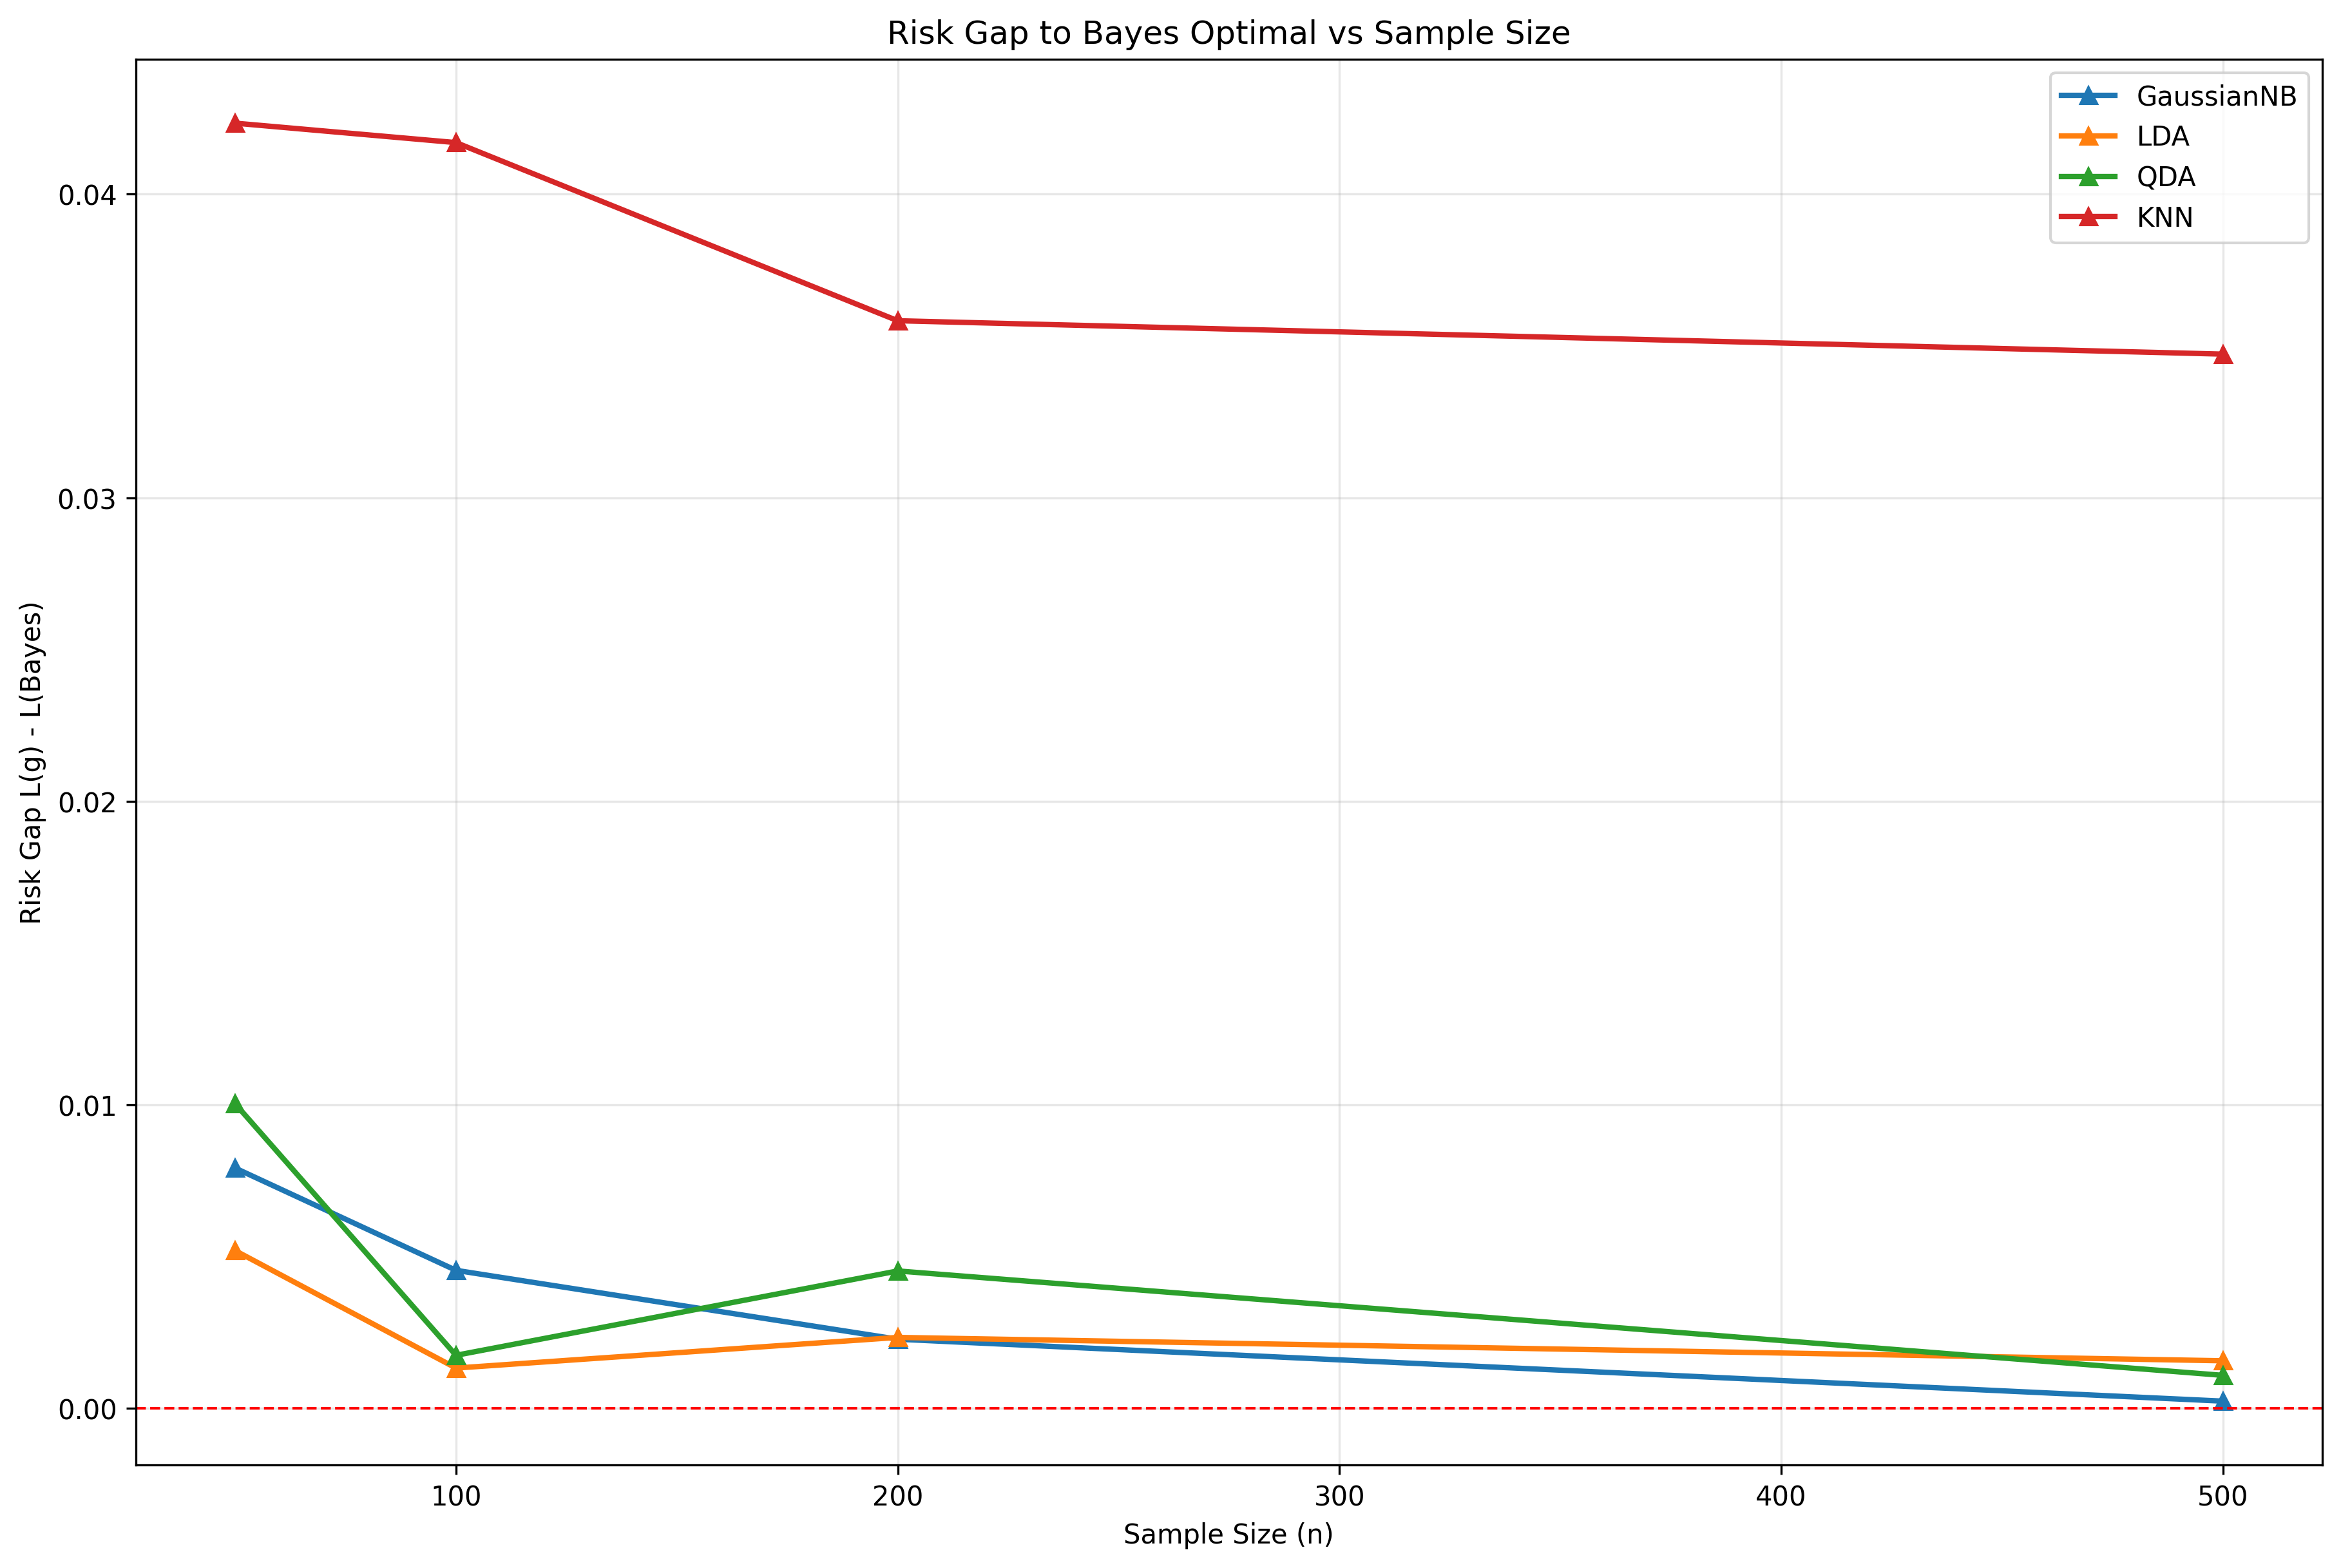
\includegraphics[width=0.60\textwidth]{figures/risk_gaps.png}
    \caption{Brechas $L(g)-L(Bayes)$ en el escenario de covarianzas iguales.}
    \label{fig:riskgap_samecov}
\end{figure}

\paragraph{Sensibilidad de k-NN.}
El clasificador \textbf{k-NN} presenta un patrón clásico de compromiso sesgo–varianza. 
Para $k=1$, logra capturar bien estructuras locales pero a costa de fronteras irregulares y alto riesgo de sobreajuste. 
En contraste, valores grandes de $k$ suavizan demasiado la frontera y generan mayor sesgo. 
La Figura~\ref{fig:knn_samecov} muestra que con valores intermedios (ej. $k=5$) se obtiene un compromiso razonable, 
aunque sin alcanzar el desempeño de LDA ni de Bayes en este escenario lineal.

\begin{figure}[H]
    \centering
    \includegraphics[width=0.60\textwidth]{figures/knn_study_balanced.png}
    \caption{Riesgo de k-NN en función de $k$ con covarianzas iguales y clases balanceadas.}
    \label{fig:knn_samecov}
\end{figure}

\paragraph{Validación vs.\ riesgo verdadero.}
La validación cruzada estratificada estima de forma bastante precisa el riesgo de LDA y Naive Bayes, 
reflejando correctamente su cercanía al clasificador de Bayes. 
En QDA y k-NN, sin embargo, se observa mayor variabilidad en las estimaciones de CV cuando $n$ es pequeño, 
lo que resalta la importancia de replicar simulaciones para obtener resultados estables.

En resumen, LDA es óptimo en covarianzas iguales, reproduciendo el desempeño del clasificador de Bayes. Naive Bayes se mantiene competitivo, aunque con un sesgo leve debido a suponer independencia. Además QDA no aporta ventaja en este escenario y puede ser contraproducente en muestras pequeñas. Por último, k-NN depende fuertemente de $k$, mostrando sobreajuste para $k$ pequeños y sesgo para $k$ grandes, sin alcanzar a LDA en este contexto.

\subsection*{Escenario 2: Clases balanceadas con covarianzas distintas}

En este escenario se mantienen priors balanceados $\pi_0=\pi_1=0.5$, pero ahora se asignan matrices de covarianza diferentes a cada clase. 
Por teoría, el clasificador de Bayes coincide con QDA, lo que convierte a este escenario en un banco de prueba natural para validar su desempeño.

\paragraph{Desempeño comparativo.}
La Figura~\ref{fig:risk_diffcov} muestra el comportamiento de los clasificadores bajo esta configuración. 
Tal como se esperaba, \textbf{QDA reproduce casi exactamente el clasificador de Bayes}, alcanzando riesgos promedio muy similares y con brechas $L(\text{QDA})-L(\text{Bayes})$ cercanas a cero (véase Figura~\ref{fig:riskgap_diffcov}). 
Esto confirma que QDA es el método paramétrico adecuado cuando las clases presentan estructuras de dispersión distintas.

\begin{figure}[H]
    \centering
    \includegraphics[width=0.68\textwidth]{figures/classifier_comparison_balanced_distinct_cov.png}
    \caption{Comparación de clasificadores con covarianzas distintas y clases balanceadas.}
    \label{fig:risk_diffcov}
\end{figure}

\begin{figure}[H]
    \centering
    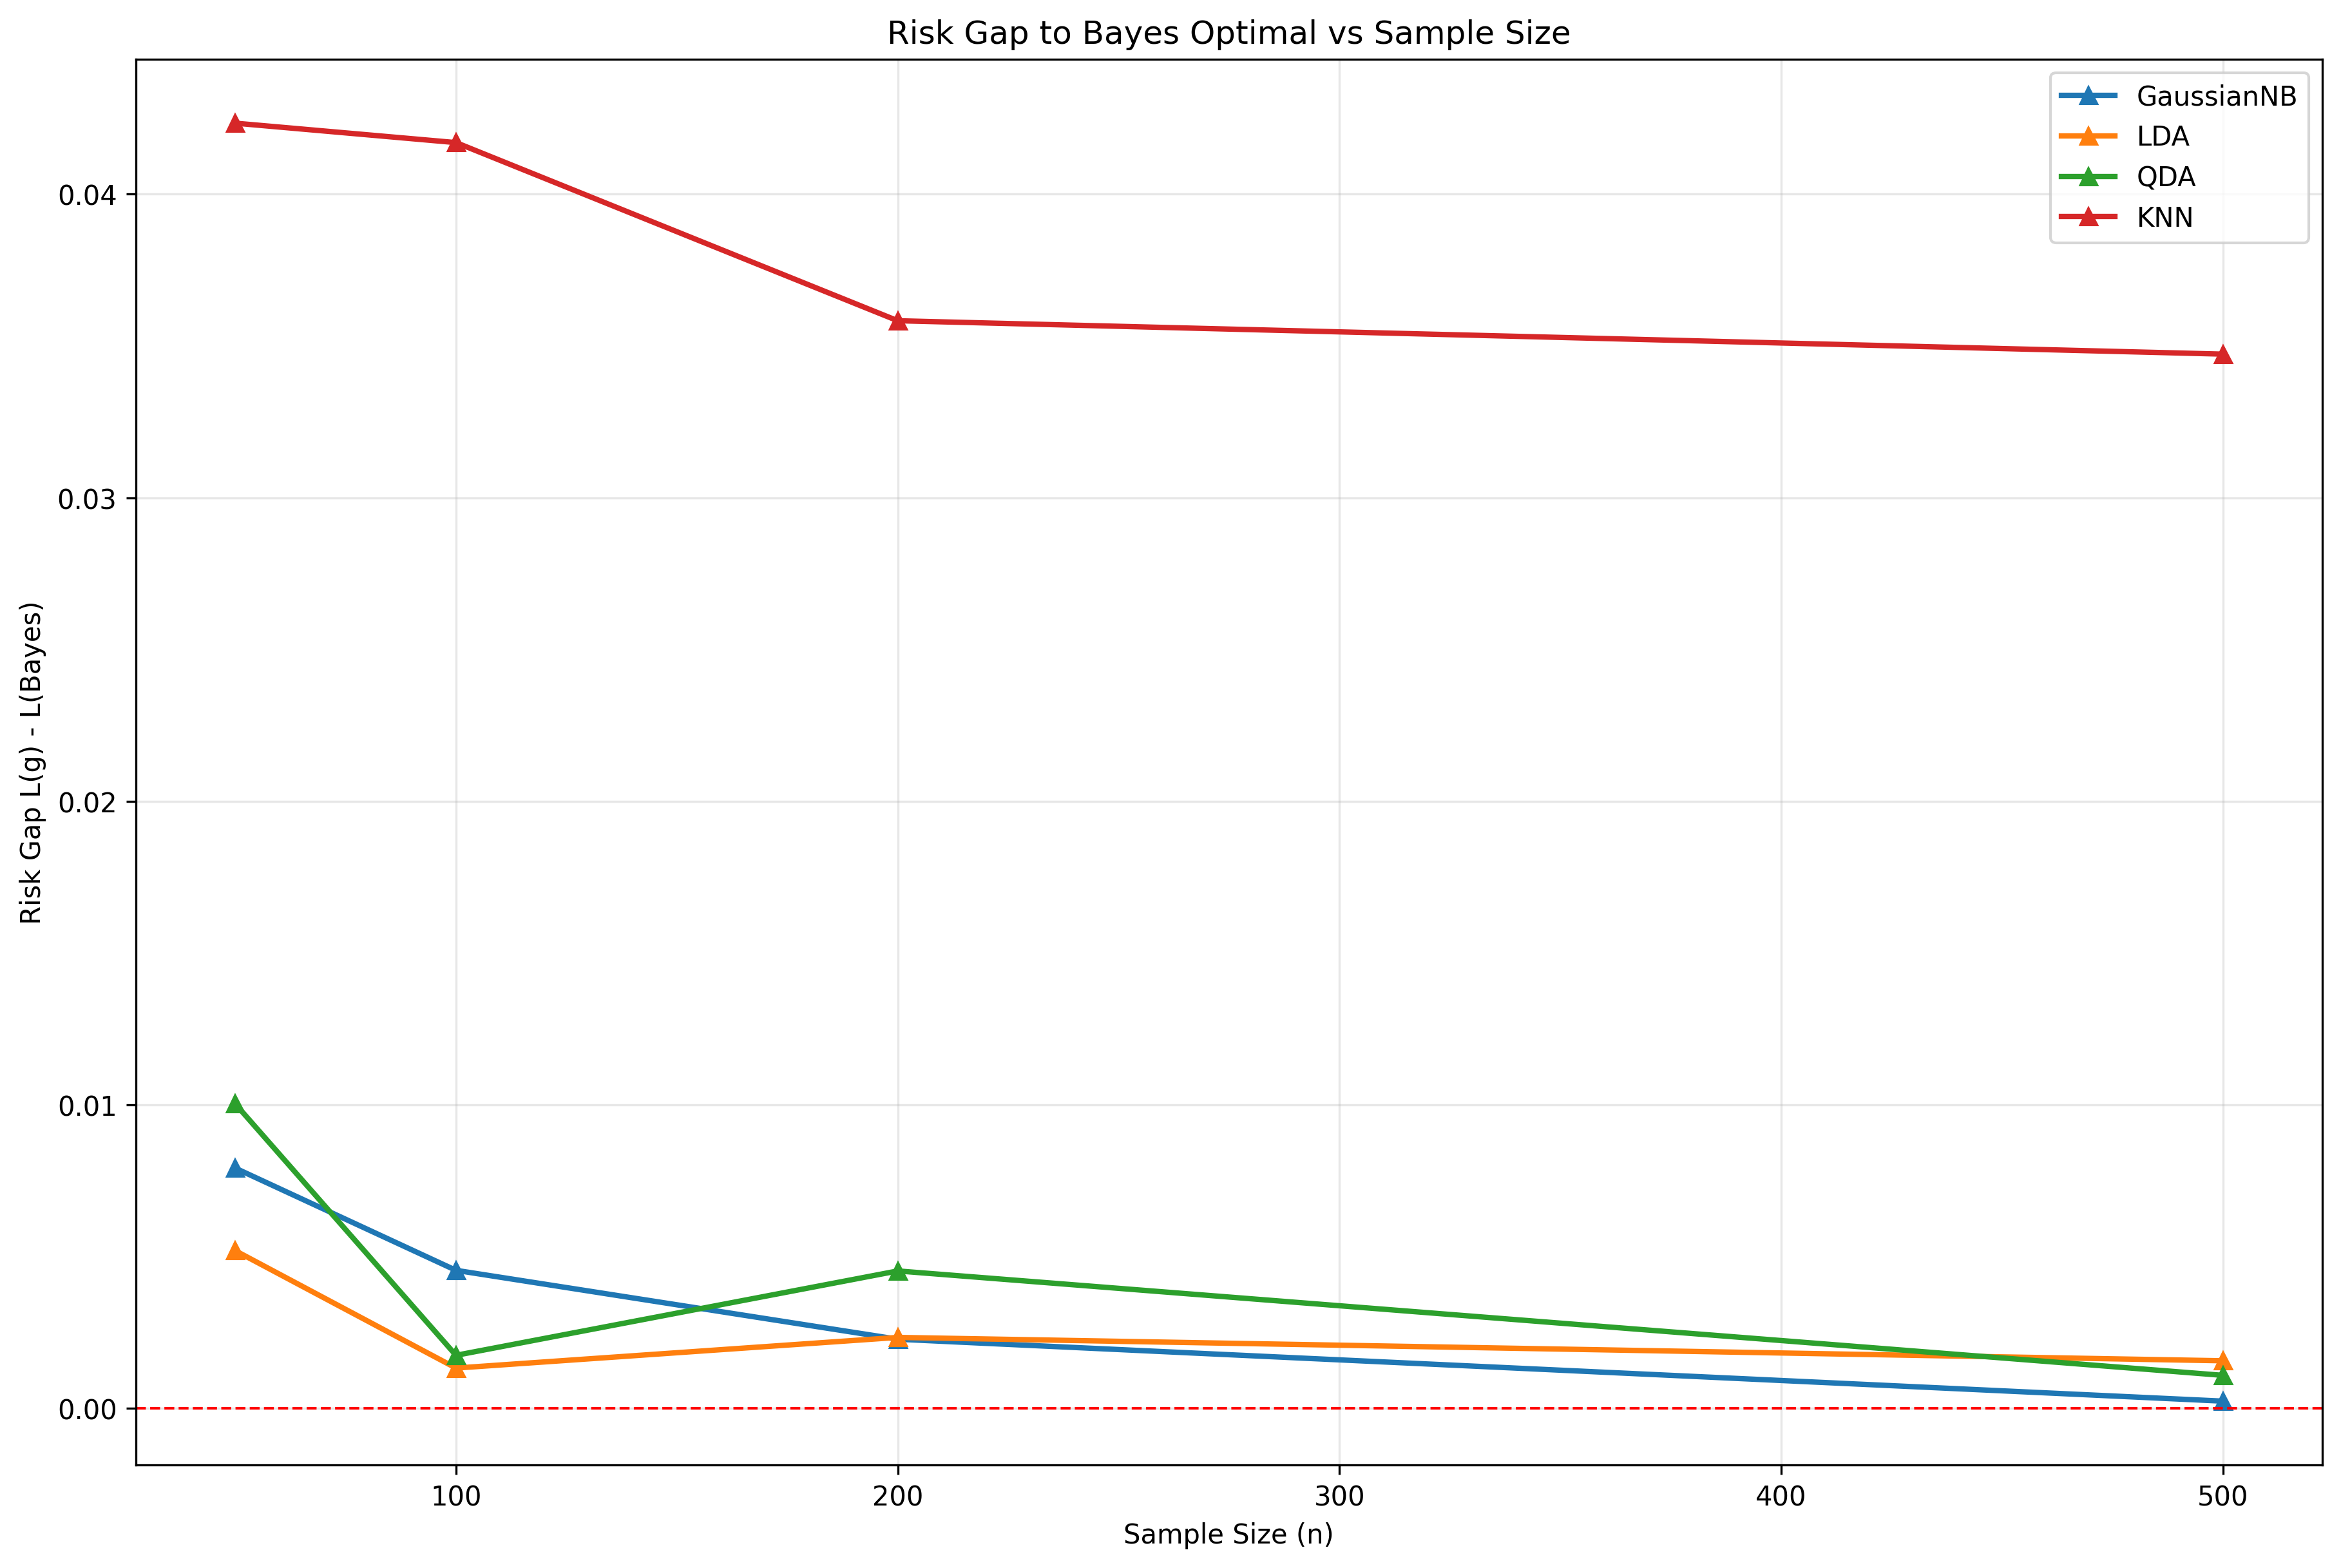
\includegraphics[width=0.55\textwidth]{figures/risk_gaps.png}
    \caption{Brechas $L(g)-L(Bayes)$ en el escenario de covarianzas distintas.}
    \label{fig:riskgap_diffcov}
\end{figure}

En contraste, \textbf{LDA presenta un sesgo sistemático positivo}, al imponer una frontera lineal en un problema cuya frontera óptima es cuadrática. 
Aunque LDA mejora conforme aumenta $n$, nunca alcanza el desempeño de QDA ni de Bayes, ya que su supuesto estructural es incorrecto.

El \textbf{Naive Bayes} mantiene un comportamiento intermedio: al ignorar correlaciones, obtiene un riesgo superior al de QDA pero en algunos casos comparable al de LDA. 
Esto lo posiciona como un método simplificado que puede ser útil cuando la correlación no es muy fuerte, aunque con pérdidas respecto al óptimo.

\paragraph{Sensibilidad de k-NN.}
El clasificador \textbf{k-NN} nos muestra un patrón dependiente tanto del tamaño de muestra como de $k$. 
La Figura~\ref{fig:knn_diffcov} muestra que con $k$ pequeños el riesgo es muy variable (alta varianza por sobreajuste), mientras que con $k$ grandes se observa sesgo elevado (fronteras demasiado suavizadas). 
En general, valores intermedios de $k$ logran un desempeño competitivo, pero aún así se mantienen por encima de QDA.

\begin{figure}[H]
    \centering
    \includegraphics[width=0.60\textwidth]{figures/knn_study_balanced.png}
    \caption{Riesgo de k-NN en función de $k$ con covarianzas distintas y clases balanceadas.}
    \label{fig:knn_diffcov}
\end{figure}

\paragraph{Validación vs.\ riesgo verdadero.}
La comparación entre validación cruzada y riesgo verdadero revela que:
\begin{itemize}
    \item Para \textbf{QDA}, las estimaciones de CV se alinean estrechamente con el riesgo de Bayes, evidenciando baja varianza y sesgo mínimo en la validación.
    \item En \textbf{LDA} y \textbf{Naive Bayes}, la validación tiende a sobrestimar ligeramente el error, reflejando la falta de ajuste estructural en este escenario.
    \item En \textbf{k-NN}, la validación muestra mayor dispersión, especialmente en $n$ pequeños y valores extremos de $k$.
\end{itemize}

En resumen, obtuvimos que QDA coincide con Bayes en covarianzas distintas, confirmando que es idóneo en problemas con fronteras cuadráticas.Además LDA queda rezagado por el sesgo de suponer fronteras lineales, incluso con $n$ grande. También decimos que Naive Bayes es aceptable, pero pierde rendimiento cuando las correlaciones son relevantes.Por último, k-NN depende fuertemente de $k$ y $n$; aunque puede ser competitivo con $n$ grande, rara vez iguala el desempeño de QDA.


\subsection*{Escenario 3: Clases desbalanceadas con covarianzas iguales}

En este escenario se fijaron priors desbalanceados, típicamente $\pi_0=0.8$ y $\pi_1=0.2$, manteniendo covarianzas idénticas para ambas clases. 
De acuerdo con la teoría, el clasificador de Bayes coincide con LDA, pero la frontera de decisión se desplaza hacia la clase minoritaria debido al ajuste por priors. 
Este escenario permite analizar cómo responden los clasificadores a situaciones comunes en la práctica, donde la clase positiva (evento de interés) es poco frecuente.

\paragraph{Desempeño comparativo.}
La Figura~\ref{fig:risk_unbal_samecov} muestra los resultados de los métodos bajo este escenario. 
\textbf{LDA mantiene un riesgo muy cercano al de Bayes}, ya que ambos se ajustan correctamente al desbalance mediante la incorporación de las probabilidades a priori. 
En consecuencia, las brechas $L(\text{LDA})-L(\text{Bayes})$ permanecen cercanas a cero (véase Figura~\ref{fig:riskgap_unbal_samecov}).

\begin{figure}[H]
    \centering
    \includegraphics[width=0.65\textwidth]{figures/classifier_comparison_unbalanced_same_cov.png}
    \caption{Comparación de clasificadores con covarianzas iguales y clases desbalanceadas.}
    \label{fig:risk_unbal_samecov}
\end{figure}

\begin{figure}[H]
    \centering
    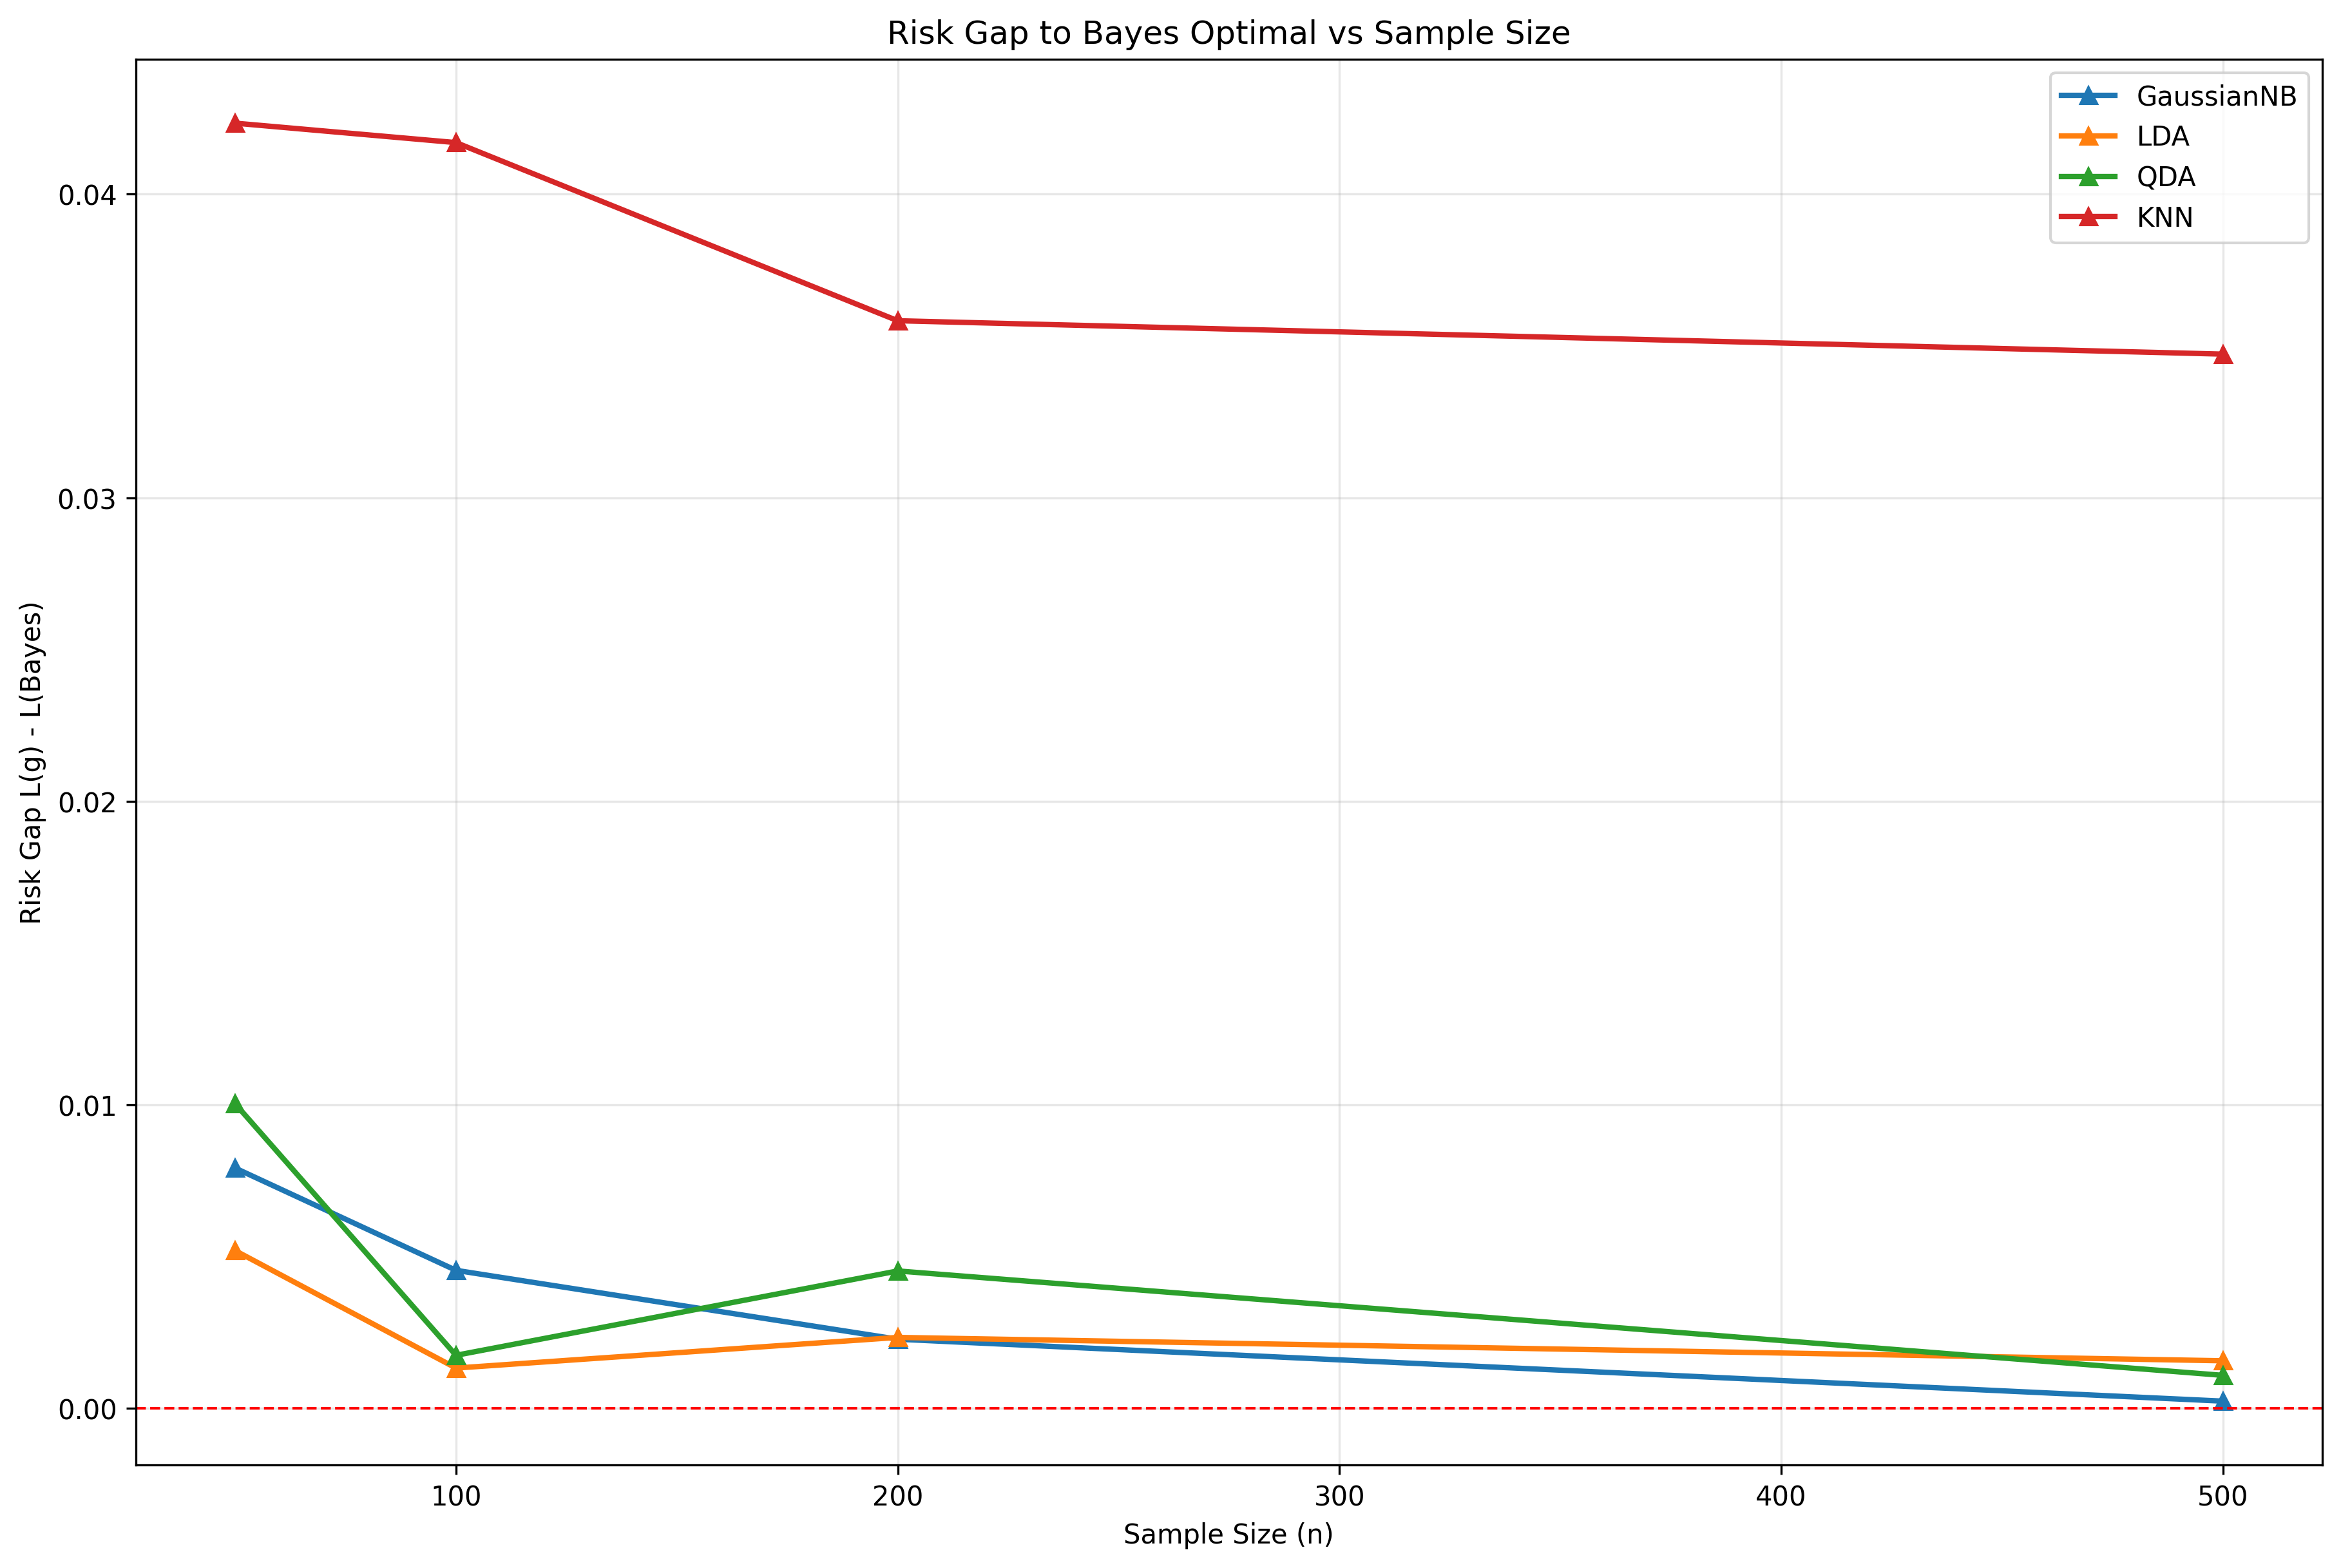
\includegraphics[width=0.60\textwidth]{figures/risk_gaps.png}
    \caption{Brechas $L(g)-L(Bayes)$ en el escenario de covarianzas iguales y desbalance.}
    \label{fig:riskgap_unbal_samecov}
\end{figure}

El \textbf{Naive Bayes} muestra un sesgo adicional frente a LDA, en parte debido a suponer independencia condicional, 
pero también porque su estimación de las probabilidades a priori es más sensible al desbalance cuando $n$ es pequeño. 
Aun así, para tamaños de muestra grandes, converge hacia un riesgo comparable al de LDA, aunque siempre ligeramente superior.

\textbf{QDA} vuelve a sufrir de varianza alta con $n$ reducido, 
y en este escenario no tiene ventaja teórica sobre LDA ya que las covarianzas son iguales. 
Esto se refleja en brechas positivas $L(\text{QDA})-L(\text{Bayes})$ más marcadas para tamaños muestrales bajos.

\paragraph{Sensibilidad de k-NN.}
El clasificador \textbf{k-NN} resulta particularmente sensible al desbalance: 
al basarse en vecinos cercanos, tiende a favorecer la clase mayoritaria, 
lo cual incrementa el riesgo de error en la clase minoritaria. 
La Figura~\ref{fig:knn_unbal_samecov} ilustra este efecto: aunque $k$ intermedios mejoran la estabilidad, 
el sesgo hacia la clase mayoritaria es evidente y limita su desempeño global frente a LDA.

\begin{figure}[H]
    \centering
    \includegraphics[width=0.60\textwidth]{figures/knn_study_unbalanced.png}
    \caption{Riesgo de k-NN en función de $k$ con covarianzas iguales y clases desbalanceadas.}
    \label{fig:knn_unbal_samecov}
\end{figure}

\paragraph{Validación vs.\ riesgo verdadero.}
La validación cruzada estratificada refleja bien el riesgo de Bayes y LDA, incluso bajo desbalance, 
gracias a que respeta las proporciones de clase en cada pliegue. 
No obstante, en k-NN y QDA se observa mayor variabilidad en las estimaciones de CV, 
lo que refuerza la necesidad de usar múltiples réplicas para obtener conclusiones confiables.

En resumen, LDA sigue siendo óptimo bajo covarianzas iguales, ajustando correctamente la frontera al desbalance de priors.Mientras que Naive Bayes es más sensible al desbalance, pero se estabiliza con muestras grandes. QDA no aporta ventaja en este escenario, y puede tener desempeño peor que LDA.Por último, k-NN se ve afectado por el desbalance, ya que la mayoría de los vecinos suelen pertenecer a la clase mayoritaria, limitando su capacidad de detectar la clase minoritaria.

\subsection*{Escenario 4: Clases desbalanceadas con covarianzas distintas}

En este escenario se combinan dos dificultades: un desbalance en las probabilidades a priori 
(típicamente $\pi_0=0.8$ y $\pi_1=0.2$) y matrices de covarianza distintas para cada clase. 
Por teoría, el clasificador de Bayes coincide con QDA, pero la frontera óptima se ve desplazada hacia la clase mayoritaria 
debido al ajuste por priors. Este es el escenario más exigente, pues introduce simultáneamente sesgo estructural y 
riesgo de varianza en la estimación de parámetros.

\paragraph{Desempeño comparativo.}
La Figura~\ref{fig:risk_unbal_diffcov} muestra los resultados de los clasificadores bajo esta configuración. 
\textbf{QDA reproduce de manera más cercana al clasificador de Bayes}, aunque su varianza en $n$ pequeños es más evidente que en escenarios balanceados. 
Las brechas $L(\text{QDA})-L(\text{Bayes})$ (Figura~\ref{fig:riskgap_unbal_diffcov}) confirman que, aunque QDA tiende al óptimo, 
su desempeño es menos estable cuando los datos son limitados y desbalanceados.

\begin{figure}[H]
    \centering
    \includegraphics[width=0.7\textwidth]{figures/classifier_comparison_unbalanced_distinct_cov.png}
    \caption{Comparación de clasificadores con covarianzas distintas y clases desbalanceadas.}
    \label{fig:risk_unbal_diffcov}
\end{figure}

\begin{figure}[H]
    \centering
    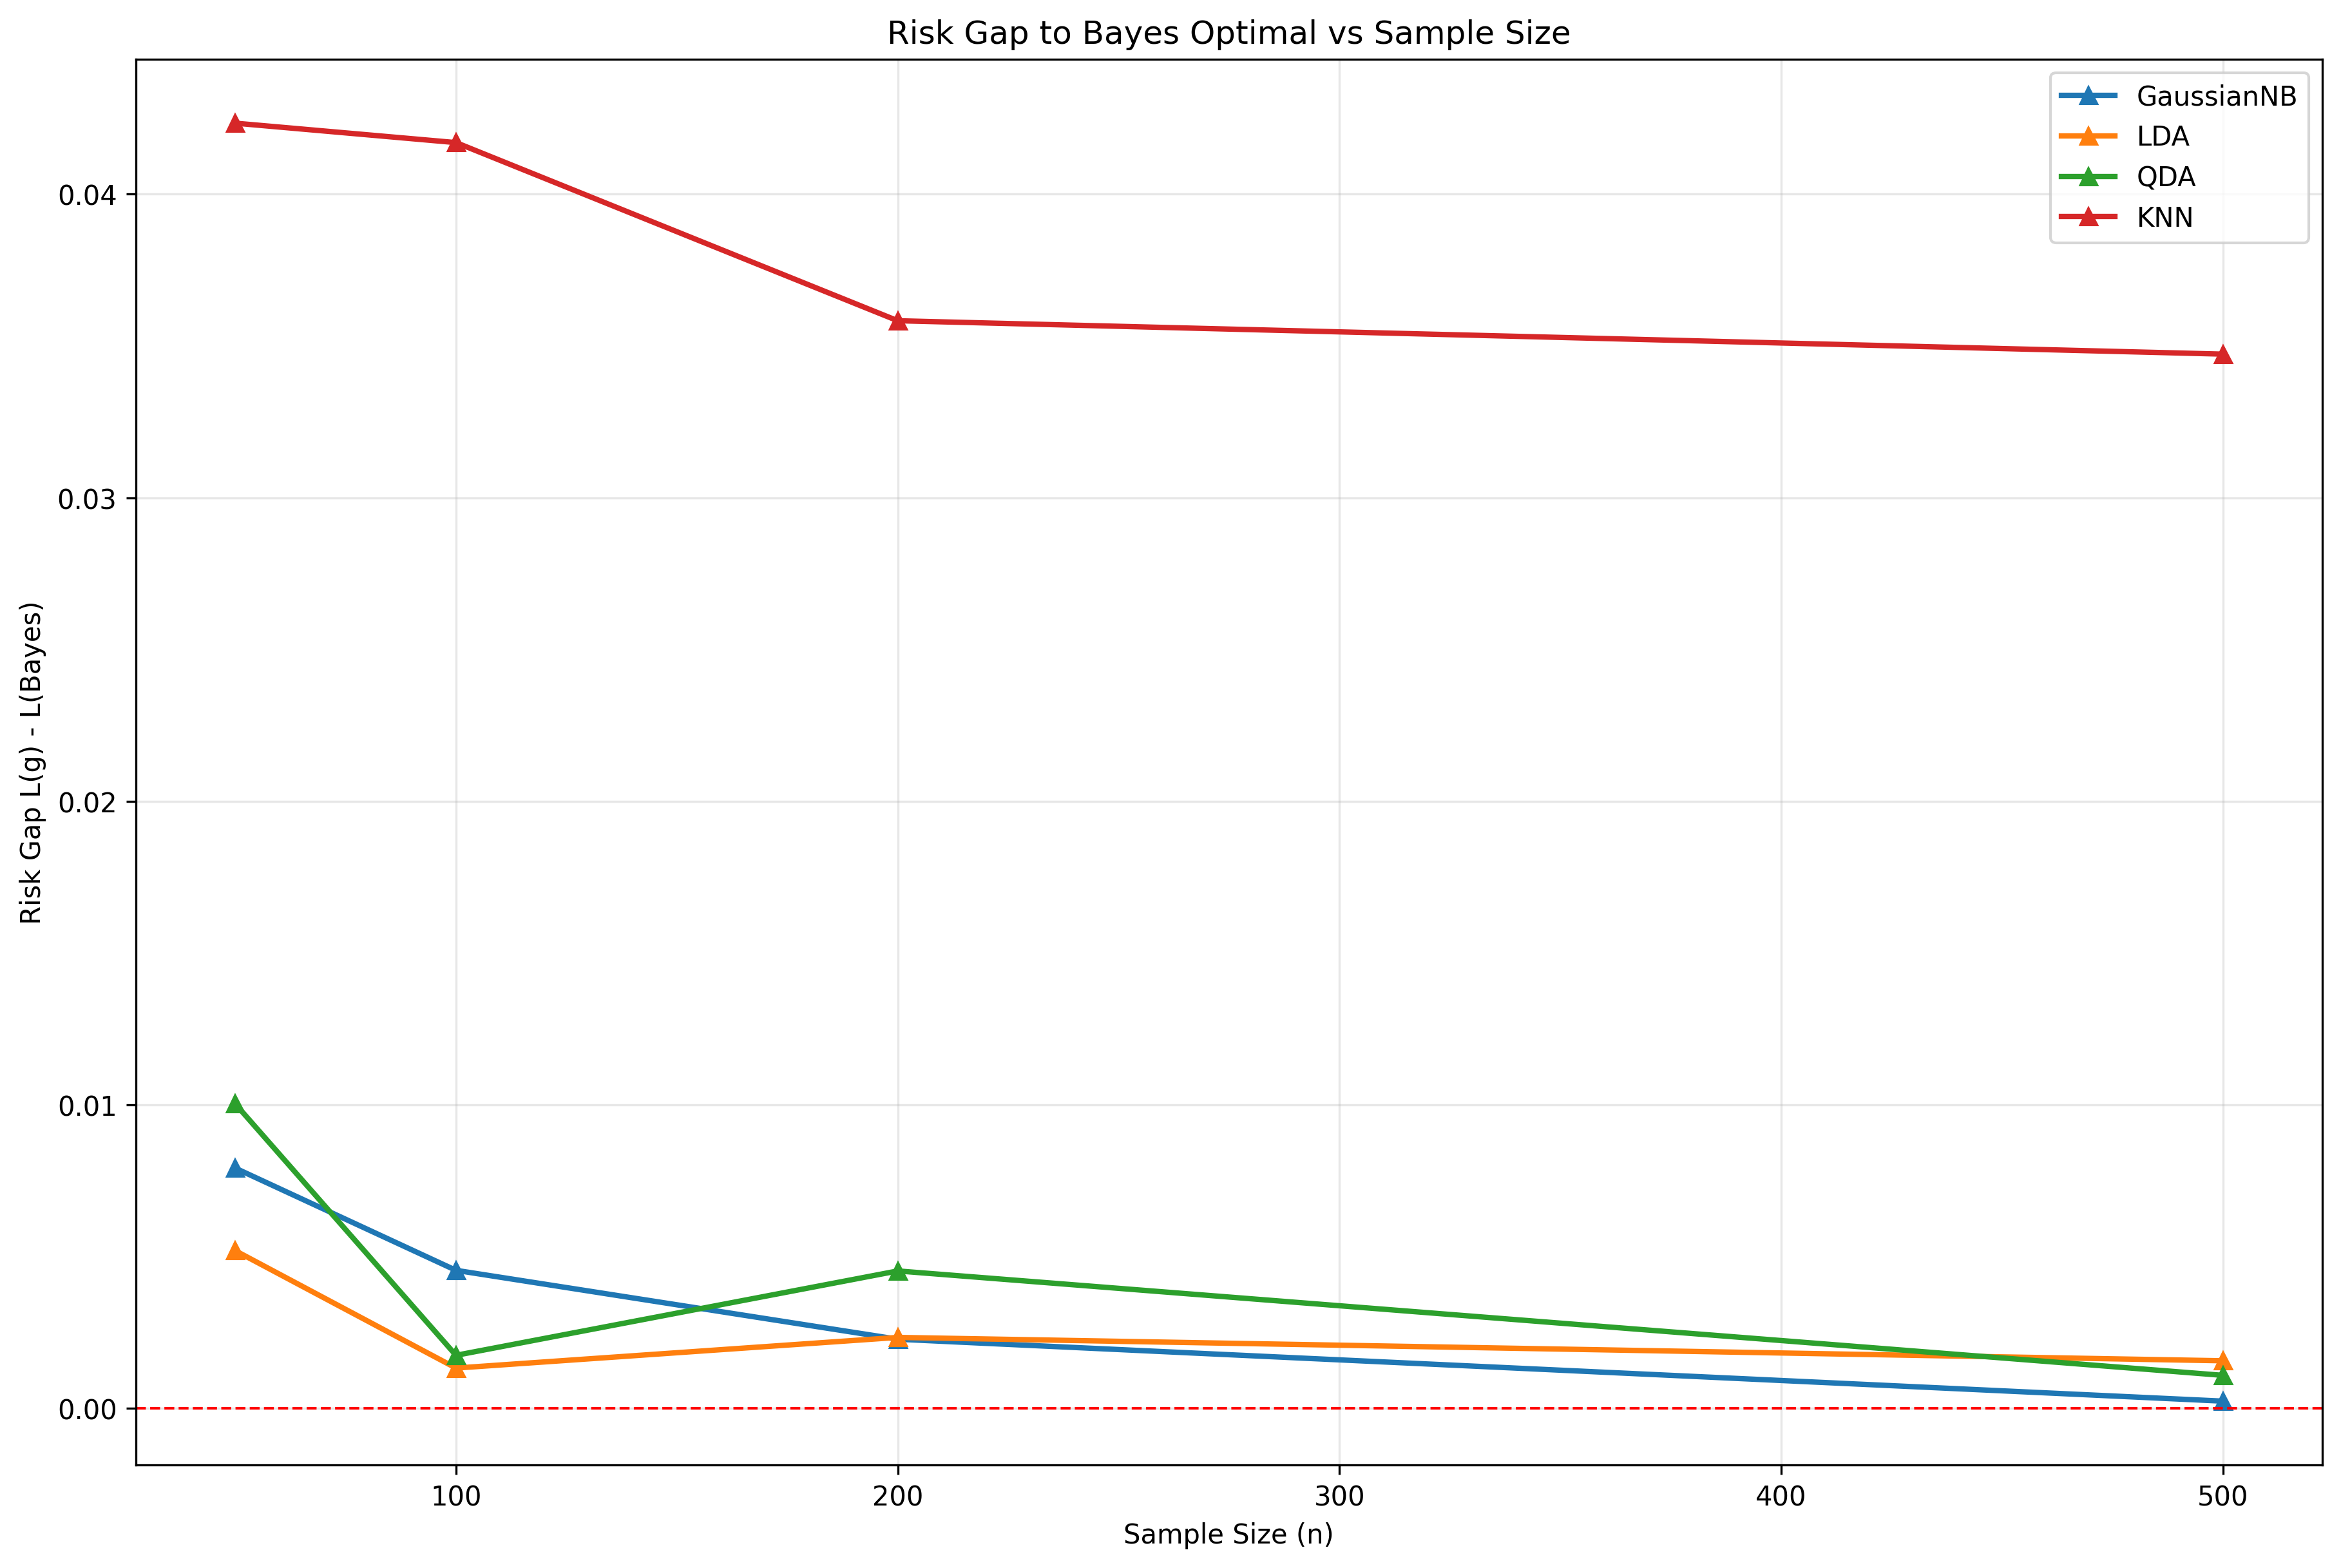
\includegraphics[width=0.60\textwidth]{figures/risk_gaps.png}
    \caption{Brechas $L(g)-L(Bayes)$ en el escenario de covarianzas distintas y desbalance.}
    \label{fig:riskgap_unbal_diffcov}
\end{figure}

En contraste, \textbf{LDA exhibe un desempeño claramente peor}, ya que impone fronteras lineales en un problema 
cuyo límite de decisión óptimo es cuadrático. El sesgo es más pronunciado que en el escenario balanceado, 
pues además se ve afectado por la asimetría de clases.

El \textbf{Naive Bayes} se muestra ineficiente en este escenario: su suposición de independencia condicional reduce aún más 
la capacidad de capturar correlaciones entre variables, y el desbalance acentúa su tendencia a favorecer la clase mayoritaria. 
Su riesgo se ubica por encima de QDA y en algunos casos incluso de LDA.

\paragraph{Sensibilidad de k-NN.}
El clasificador \textbf{k-NN} presenta las mayores dificultades en este escenario. 
El desbalance provoca que la mayoría de los vecinos pertenezcan a la clase más común, 
incrementando drásticamente la tasa de error en la clase minoritaria. 
La Figura~\ref{fig:knn_unbal_diffcov} muestra que, incluso con $k$ calibrados, el rendimiento de k-NN rara vez se aproxima al de QDA. 
Este hallazgo evidencia la vulnerabilidad de métodos basados en distancias en situaciones de desbalance severo.

\begin{figure}[H]
    \centering
    \includegraphics[width=0.60\textwidth]{figures/knn_study_unbalanced.png}
    \caption{Riesgo de k-NN en función de $k$ con covarianzas distintas y clases desbalanceadas.}
    \label{fig:knn_unbal_diffcov}
\end{figure}

\paragraph{Validación vs.\ riesgo verdadero.}
En este escenario complejo, la validación cruzada presenta una mayor dispersión, especialmente en QDA y k-NN. 
Si bien en promedio las estimaciones de CV siguen la tendencia del riesgo verdadero, 
los intervalos de variabilidad son más amplios, lo cual indica que con muestras pequeñas el desempeño estimado puede ser inestable. 
Esto resalta la importancia de usar múltiples réplicas Monte Carlo para obtener conclusiones robustas.

Por lo tanto, QDA es el método más adecuado, al coincidir con Bayes, pero su desempeño se ve afectado por la varianza en muestras pequeñas y el desbalance de clases.
Pero, LDA y Naive Bayes se ven penalizados tanto por el sesgo estructural (fronteras lineales o independencia condicional) como por la asimetría de clases. k-NN sufre significativamente en condiciones de desbalance, mostrando alta tasa de error en la clase minoritaria, incluso tras calibrar $k$. Este escenario ilustra el peor caso para la mayoría de los clasificadores, y subraya la necesidad de considerar tanto la estructura de covarianzas como el balance de clases en aplicaciones reales.



\subsection*{Validación cruzada vs. riesgo verdadero}

Además de los resultados por escenario, se evaluó la capacidad de la validación cruzada para aproximar el riesgo verdadero de cada clasificador. 
La Figura~\ref{fig:val_comparison} resume esta comparación en distintos contextos experimentales.

\begin{figure}[H]
    \centering
    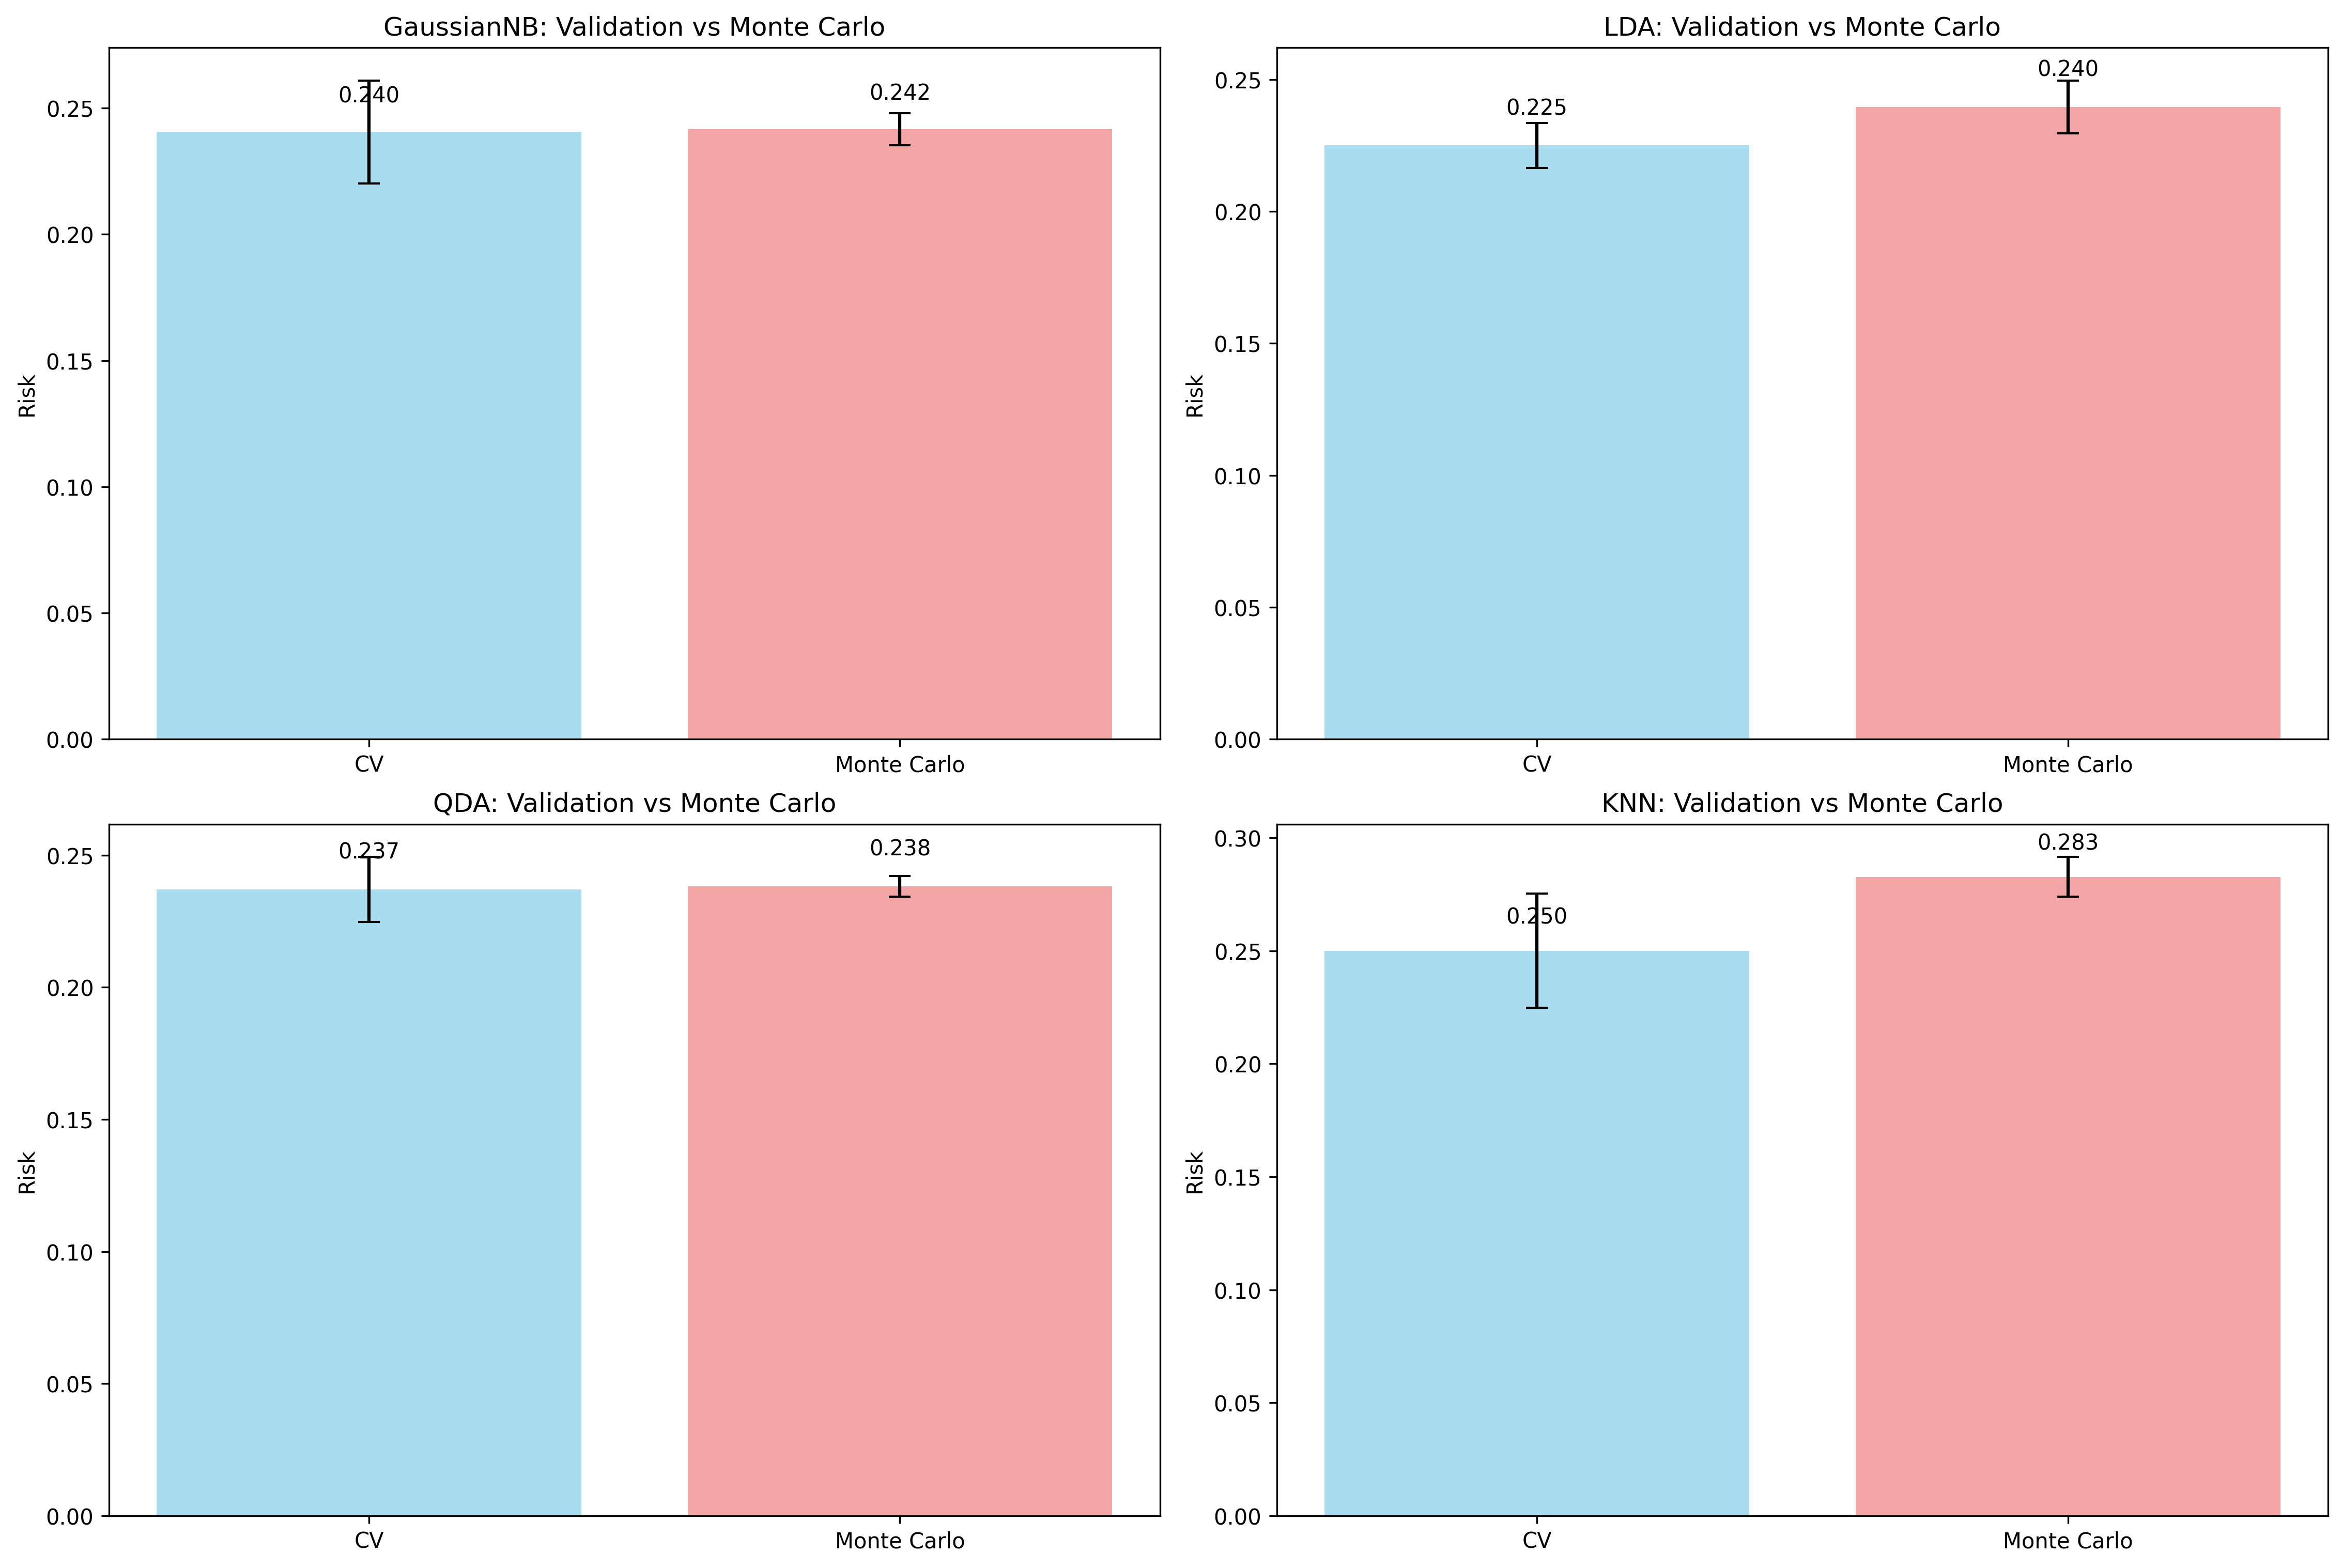
\includegraphics[width=0.70\textwidth]{figures/validation_comparison.png}
    \caption{Comparación entre riesgo estimado por validación cruzada (CV) y riesgo verdadero (Monte Carlo) en distintos escenarios.}
    \label{fig:val_comparison}
\end{figure}

Los resultados muestran que:
\begin{itemize}
    \item En \textbf{LDA} y \textbf{Naive Bayes}, la validación cruzada ofrece estimaciones muy cercanas al riesgo verdadero, incluso con tamaños de muestra moderados.
    \item En \textbf{QDA}, la validación refleja adecuadamente la tendencia general, aunque su varianza aumenta cuando $n$ es pequeño.
    \item En \textbf{k-NN}, las estimaciones de CV son mucho más variables, lo que sugiere que este método es más sensible a la partición de los datos y requiere más réplicas para estabilizarse.
\end{itemize}

En conjunto, la validación cruzada se confirma como un estimador confiable del riesgo, aunque con sesgos y varianzas que dependen del clasificador y de las condiciones del problema.




\section*{Conclusiones}

El análisis computacional mediante simulaciones permitió contrastar el desempeño de distintos clasificadores supervisados frente al clasificador óptimo de Bayes en escenarios controlados. 
Los resultados obtenidos refuerzan las propiedades teóricas de cada método y aportan evidencia empírica sobre sus ventajas y limitaciones prácticas.

En primer lugar, se verificó que \textbf{LDA y QDA coinciden con Bayes} en los escenarios donde sus supuestos son correctos: covarianzas iguales para LDA y covarianzas distintas para QDA. 
Esto nos confirma que, cuando los supuestos del modelo se cumplen, los clasificadores paramétricos alcanzan el desempeño óptimo. 
No obstante, observamos que \textbf{QDA es más sensible al tamaño muestral}, presentando alta varianza en situaciones de datos escasos.

En segundo lugar, \textbf{Naive Bayes} se mostró como una alternativa competitiva en escenarios con correlaciones bajas, aunque siempre con un riesgo ligeramente mayor al de LDA o QDA. 
Su simplicidad y robustez lo hacen atractivo, pero la suposición de independencia condicional limita su capacidad de alcanzar al óptimo.

Por otra parte, el \textbf{criterio de Fisher} resultó útil como aproximación lineal rápida, capturando buena parte de la separabilidad en escenarios simples, aunque su reducción a una dimensión implica pérdidas cuando la frontera es no lineal.

El \textbf{k-NN} exhibió un comportamiento altamente dependiente de $k$ y del tamaño muestral. 
Con valores intermedios de $k$ y muestras grandes logró un desempeño razonable, pero rara vez igualó a los métodos paramétricos. 
Además, se mostró especialmente vulnerable al desbalance de clases, donde tendió a favorecer a la clase mayoritaria.

Finalmente, la comparación entre \textbf{riesgo verdadero y riesgo estimado por validación} mostró que la validación cruzada estratificada es, en general, un buen estimador del desempeño real, 
con sesgos pequeños para LDA y Naive Bayes, pero con mayor variabilidad para QDA y k-NN en muestras reducidas. 
Esto destaca la importancia de considerar tanto el sesgo como la varianza de los estimadores de riesgo al evaluar clasificadores.

En conjunto, las simulaciones evidencian que:
\begin{itemize}
    \item Los métodos paramétricos alcanzan el óptimo cuando sus supuestos son válidos, pero pueden deteriorarse cuando éstos se violan.
    \item Los métodos no paramétricos como k-NN son más flexibles, pero requieren más datos y son sensibles al desbalance.
    \item La validación empírica, aunque aproximada, es una herramienta confiable para estimar el riesgo en la práctica, siempre que se reconozcan sus limitaciones.
\end{itemize}

Estas conclusiones ilustran cómo la teoría de clasificación estadística se traduce en la práctica computacional: 
ningún método es universalmente superior, y la elección adecuada depende de la estructura de los datos, el tamaño muestral y la naturaleza del problema. 
La simulación, al ofrecer un entorno donde la verdad es conocida, se consolida como una herramienta esencial para entender las fortalezas y debilidades de cada clasificador.


\begin{thebibliography}{9}

\bibitem{hastie}
Hastie, T., Tibshirani, R., \& Friedman, J. (2009). 
\textit{The Elements of Statistical Learning: Data Mining, Inference, and Prediction}. 
Springer Series in Statistics. (2ª ed.).  

\bibitem{james}
James, G., Witten, D., Hastie, T., \& Tibshirani, R. (2021). 
\textit{An Introduction to Statistical Learning with Applications in R and Python}. 
Springer. (2ª ed.).  

\bibitem{bishop}
Bishop, C. M. (2006). 
\textit{Pattern Recognition and Machine Learning}. 
Springer.  

\bibitem{duda}
Duda, R. O., Hart, P. E., \& Stork, D. G. (2000). 
\textit{Pattern Classification}. 
Wiley-Interscience. (2ª ed.).  

\bibitem{efron}
Efron, B., \& Tibshirani, R. J. (1993). 
\textit{An Introduction to the Bootstrap}. 
Chapman \& Hall/CRC.  

\end{thebibliography}

\end{document}